\documentclass{article}
\usepackage[utf8]{inputenc}
\usepackage{fontawesome}
\usepackage{hyperref}
\usepackage{graphicx}
\usepackage{amsmath,amssymb}
\usepackage[left=2cm,right=2cm,bottom=2cm,top=2cm]{geometry}
\usepackage{float}


\title{Arquitectura de Computadoras Lab-1}
\author{anthony.aguilar }
\date{September 2020}

\begin{document}

\maketitle
\newpage
\section*{Comentarios previos}
\begin{itemize}
    \item Dentro de la carpeta de cada pregunta hay un makefile para compilar, ejecutar, mostrar las waves y limpiar los archivos generados al finalizar.
    \item Use github\faGithub \space porque trabaje este laboratorio en 2 computadoras y necesitaba una forma de compartir los archivos entre ambas. Y el repositorio es publico para que los links adjuntos funcionen.
\end{itemize}

\section*{Ejercicio 1}
\subsection*{Explicación}
Para este ejercicio hice primero un MUX 2:1 para crear un MUX 4:1 que use para hacer un MUX 8:1 (que realmente no era necesario) para finalmente completar el MUX 16:1.
\subsection*{Código}
\faGithub \space
\href{https://github.com/warleon/Arch-lab1/tree/master/pregunta1}{https://github.com/warleon/Arch-lab1/tree/master/pregunta1}\\
make MUX\_16\_1
%\subsection*{Tabla de verdad}

%\subsection*{Mapa de Karnaugh}

%\subsection*{Ecuaciones booleanas}

\subsection*{Resultados}
\begin{figure}[h]
    \centering
    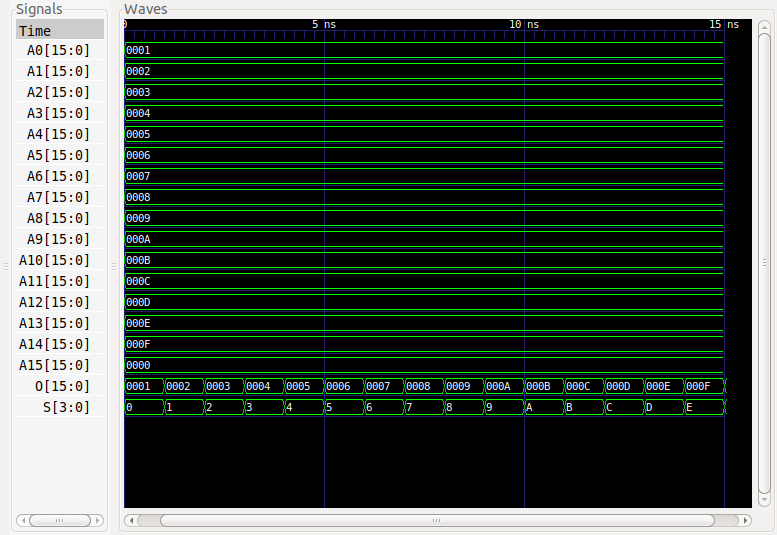
\includegraphics[scale=0.6]{fotos/resultados/arki-MUX_16_1.png}
    \caption{waves mux 16:1}
\end{figure}
\newpage

\section*{Ejercicio 2}
\subsection*{Explicación}
Para este ejercicio seguí la misma lógica del ejercicio 1 pero obviando el DEMUX 1:8.

\subsection*{Código}
\faGithub \space
\href{https://github.com/warleon/Arch-lab1/tree/master/pregunta2}{https://github.com/warleon/Arch-lab1/tree/master/pregunta2}\\
make DEMUX\_1\_16
%\subsection*{Tabla de verdad}

%\subsection*{Mapa de Karnaugh}

%\subsection*{Ecuaciones booleanas}

\subsection*{Resultados}
\begin{figure}[h]
    \centering
    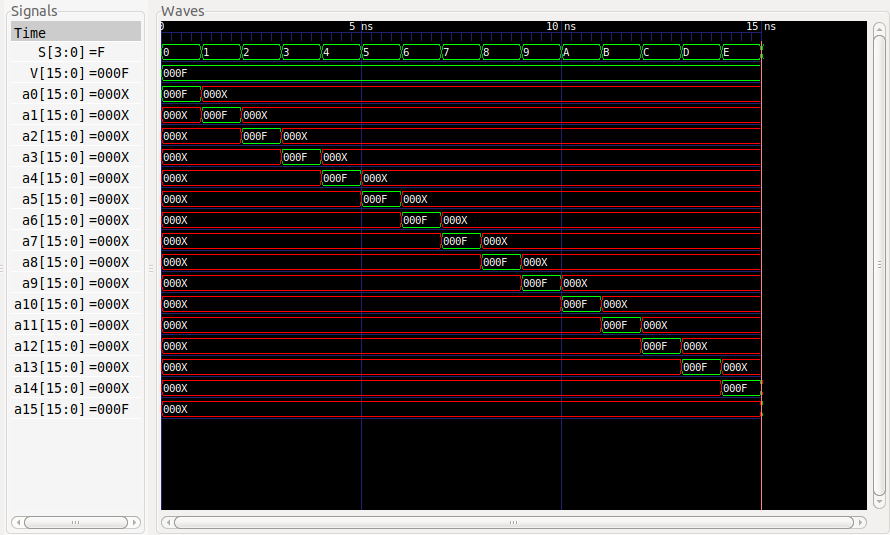
\includegraphics[scale=0.5]{fotos/resultados/arki-DEMUX_1_16.png}
    \caption{waves demux 1:16}
\end{figure}
\newpage

\section*{Ejercicio 3}
\subsection*{Explicación}
Para este ejercicio hice uso del if statement de verilog para comprobar cada caso aunque tambíen pude hacer uso del case statement (pero preferí el if).
\subsection*{Código}
\faGithub \space
\href{https://github.com/warleon/Arch-lab1/tree/master/pregunta3}{https://github.com/warleon/Arch-lab1/tree/master/pregunta3}\\
make comparador

%\subsection*{Tabla de verdad}

%\subsection*{Mapa de Karnaugh}

%\subsection*{Ecuaciones booleanas}

\subsection*{Resultados}
\begin{figure}[h]
    \centering
    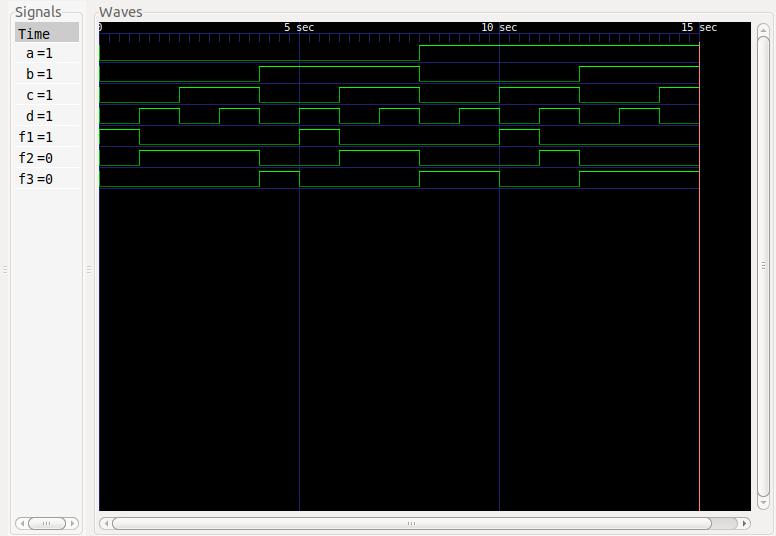
\includegraphics[scale=0.6]{fotos/resultados/arki-COMPARADOR.png}
    \caption{waves comparador}
\end{figure}
\newpage

\section*{Ejercicio 4}
\subsection*{Explicación}
Para este ejercicio sí use kmaps e hice una implementación vehavioral.
\subsection*{Código}
\faGithub \space
\href{https://github.com/warleon/Arch-lab1/tree/master/pregunta4}{https://github.com/warleon/Arch-lab1/tree/master/pregunta4}\\
make decimal

%\subsection*{Tabla de verdad}

\subsection*{Mapa de Karnaugh}
\begin{figure}[h]
    \centering

    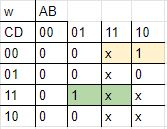
\includegraphics{fotos/kmaps/kmap1-lab1-arqui.JPG}
    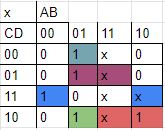
\includegraphics{fotos/kmaps/kmap2-lab1-arqui.JPG}

   
    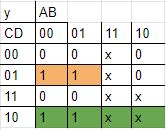
\includegraphics{fotos/kmaps/kmap3-lab1-arqui.JPG}
    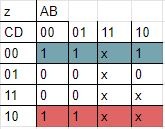
\includegraphics{fotos/kmaps/kmap4-lab1-arqui.JPG}
\end{figure}

\subsection*{Ecuaciones booleanas}
$W=A.\overline{D}+B.C.D$\\
$X=\overline{B}.C.D+B.\overline{C}.D+\overline{A}.B.\overline{D}+A.C.\overline{D}$\\
$Y=\overline{A}.\overline{C}.D+C.\overline{D}$\\
$Z=\overline{C}.\overline{D}+C.\overline{D}$\\

\subsection*{Resultados}
\begin{figure}[h]
    \centering
    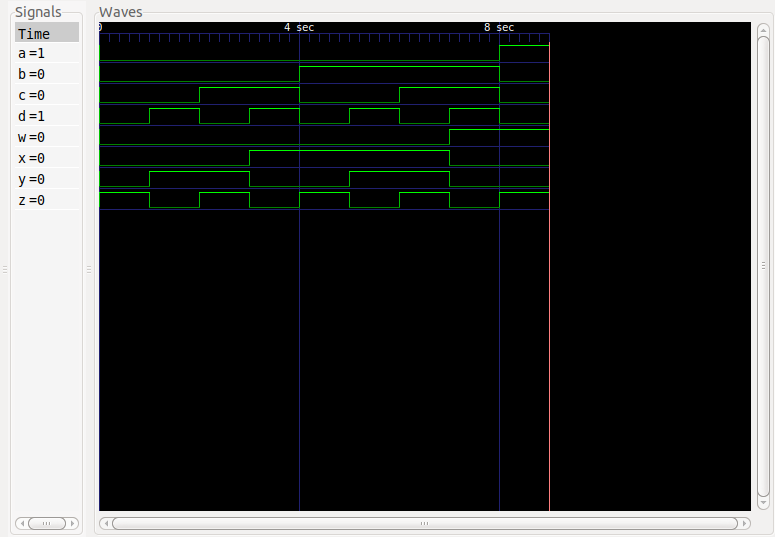
\includegraphics[scale=0.6]{fotos/resultados/arki-DECIMAL.png}
    \caption{waves BCD}
\end{figure}


\end{document}
